% !TEX encoding = UTF-8
% !TEX TS-program = pdflatex
% !TEX root = ../Tesi.tex
% !TEX spellcheck = it-IT

%************************************************
\chapter{Acustica di san Luca: ricostruzione e perdita}
\label{cap:acustica}
%************************************************

%\begin{flushright}{\slshape
%  L'enigma che risuona dalle mascelli feroci della vergine \\
%  \medskip
%    --- Pindaro
%\end{flushright}

%-preludio e cenno storico
%
%-environment
%
%-struttura
%
%
Qui, l’incedere di una risonanza è legata ad un corpo/luogo, lentamente mutabile:
uno spazio che è memoria di superficie. Abitare questo ascolto è stato il primo
passo della scrittura, il formalizzarsi e il perdersi di una molteplice voce,
abitante abitato da \emph{per sempre}. 

La scelta del luogo, dello spazio d'ascolto è il punto di partenza.
Partenza (come dipartita), della stessa scrittura strumentale tradizionale. 
Lo studio dello spazio di San Luca ha instaurato diverse relazioni che
congiungono i diversi strati di elaborazione, dalla macro alla micro-struttura.
%
%
%
%
%
\section{Coscienza di scrittura}

L'immemorialit à dell'evento scandisce sia il gesto formale che la struttura,
organizzando i contributi qualitativi del suono e la loro distribuzione
temporale e spaziale. Immemorialità dello stesso suono come strumento trasformato
e non riconducibile a:

Altezza temperata.

È volutamente ricercato nello strumento la sua oscillazione  attorno a dei
poli frequenziali (descritti successivamente), cercando la massima <<instabilità-controllata>>.
Giochi di oscillazione che intercorrono tra l’evidente parametro multifonico e la sua de-costruzione timbrica.
Lo stesso vale per i battimenti, altri importanti operatori di trasformazione.


-----fileA------



\section{Modalità di emissione omogenea}

Gradazioni controllate di soffio e suono, oltre che intonazione di aberrazioni prodotte tramite saliva e spostamento dell'imboccatura.     

\begin{figure}
\centering
{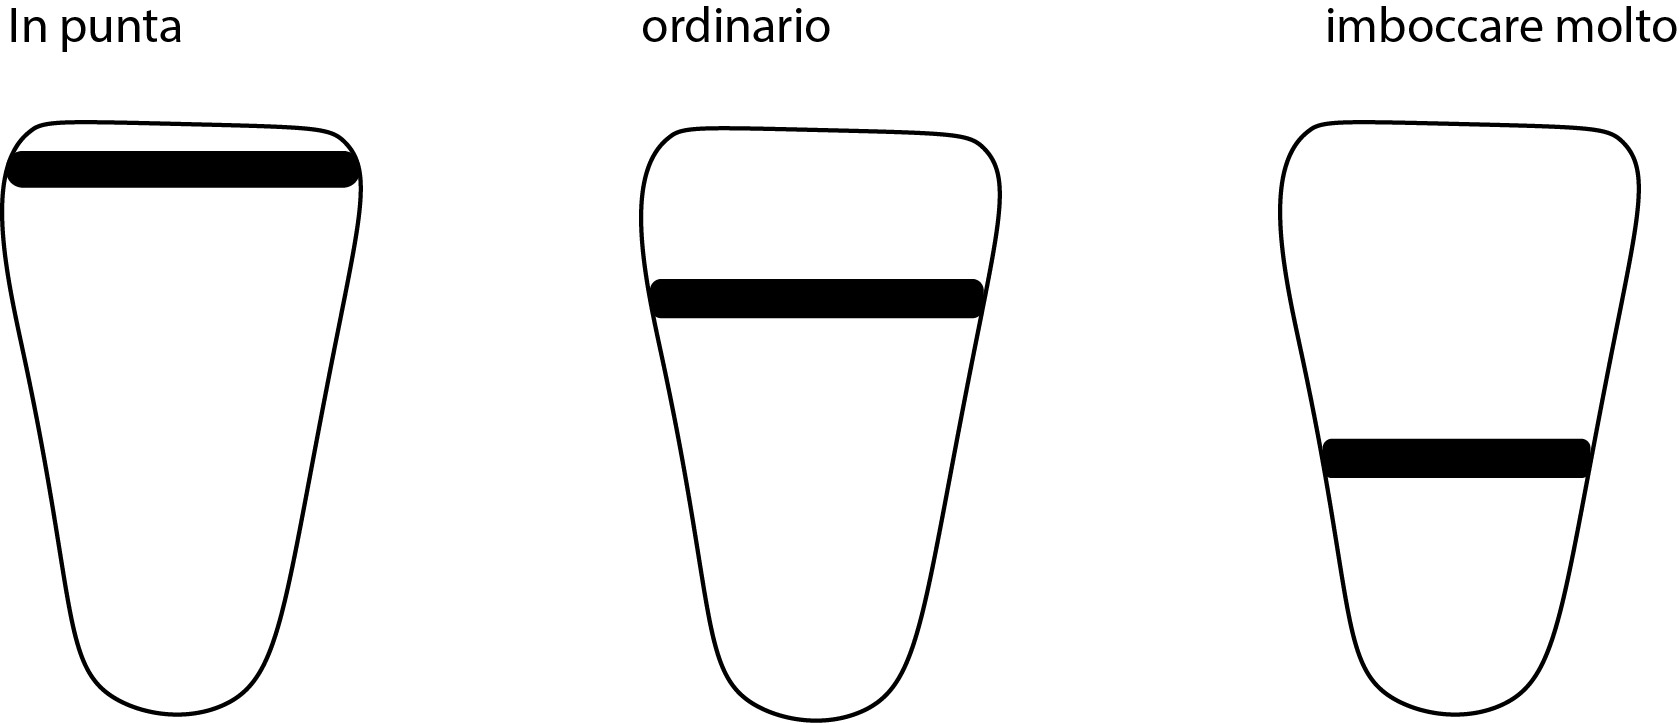
\includegraphics[width=.65\columnwidth]{sax_boc.jpg}}
\caption[Pianta S. Luca]{Schemi imboccatura}
\label{fig:tetratetra}
\end{figure}

Perché il sassofono?

Le caratteristiche cercate in questo strumento si basano sulla possibilità
di insistere su determinati fattori; il corpo/bocca dello strumentista, 
le modifiche della colonna armonica, i suoi armonici sovracuti, doppiati
e triplicati nel medesimo tempo/istante.
Il sassofono soprano rende possibile la continua modulazione tra multifonici:
una “corrente continua”,  dove il movimento lento (pensato assieme all'impronta
elettronica del luogo) permette lo stazionamento di determinate parziali
e il passaggio fluido tra differenti bicordi. È stato fondamentale lo studio
dei parziali multifonici, il loro isolamento monodico e la possibilità di 
“entrare” ed “uscire” dalla posizione di generazione multifonica.

Possiamo dividere le qualità di queste parziali in famiglie:

disegnino1* = parziali <<treshold tones>>  -  
disegnino2 = <<shadow sound>>: suoni che non possono essere i solati.
È stato posto l’accento sulle possibili aberrazioni che si pongono su ottave differenti
rispetto al suono cardine, rendendo il contenuto spettrale più instabile e ricco.
disegnino3 = instabile : alcune regioni frequenziali di multifonici presentano una
difficile risposta. Battimenti o parziali sovracuti avranno una risposta non lineare.
Si deve tendere a cercare una sorta di <<modulazione di ampiezza>>. Cercare il suono.
* i simboli sono presi dal trattato di Weiss e Netti



-----fileC-----



Conseguenziale a questo tipo di scrittura il  rapporto e la pratica con lo strumentista.
Le tecniche estese di partenza vengono dagli studi di Weiss e Netti,ma il percorso di
elaborazione, di nuova scoperta di emissione e modulazione di timbro e altezze è
stato condotto assieme al sassofonista Danilo Perticaro.

[[[[[a specchio da una parte le Qualità sonore da l'altra i suoni cardine]]]]]

Qualità sonore e trasformazione suoni cardine del brano\footnote{Alcune delle transizioni
e multifonici non si trovano nel brano. Gli schemi preparatori riportano anche lavoro a
monte rispetto allo studio con lo strumentista.  Provandoli successivamente ci siamo
resi conti di incongruenze legate alla difficolta di diteggiatura o differente
legatura di emissione (dinamiche eccessivamente differenti portavano ad non legare le posizioni)}
Ogni diteggiatura nel suo legarsi presenta un effetto di modifica non solo 
frequenziale ma dello spettro stesso delle parziali.

Assottigliamento verso i suoni sovracuti del sassofono(materiale povero spettralmente)

fileD
 
frequenza ambigua che interpola

Emissione - soffio - battimento
 
 
schema microstruttura con modifica del suono:

file E

fondamentale -parziale accrescimento-svuotamento

la logica d'uso di queste tecniche si pone lontana dagli schematismi di "effetto" che ruotano attorno all'articolazione di note.                                      

\section{Environment}

La logica spaziale proposta con la risposta all'impulso e la riproduzione tramite sistema tetraedrico, ha portato a concepire un uso delle fonti sonore che gravitano interne e all’esterno dell'ambiente della chiesa di San Luca.
 La registrazione e la riproduzione tramite sistema A-format permetteva di delineare una cartografia tridimensionale degli eventi: tramite un'azione musicale preparata sono stati controllati e scanditi i materiali suonati all'interno della chiesa: preparata in quanto si vuole nascondere il più possibile l’evento acustico dalla percezione familiare, dal suo effettivo sguardo <<concreto>>.
La logica di registrazione segue il quadrante interno alla chiesa utilizzato per gli impulsi.

\subsection{struttura del nastro}

Note 

Tre esecutori                                                            
la durata del nastro è di circa 10 minuti.
è da considerare ad libitum. Sarà chiuso il processo da parte del regista del suono.
L'incontro con la parte strumentale è fortemente aleatoria. Environment attorno all’ascoltatore, attorno allo strumentista,con un range medio-grave. È possibile riscrivere il nastro partendo dai materiali e dallo schema relativo alle dinamiche generale. Il tutto deve essere tra <<pppppp>> e <<pp>>. Mai s

MATERIALI

A= ambiente esterno alla chiesa [controllare adeguatamente il livello d'ingresso del soundfield]
B= banchi da chiesa (scricchiolio)
C= sedie
D= passi
E= voci




\subsection{Schema}

La scelta di preparare  dal vivo il materiale  concreto e non elaborarlo successivamente
è dato dal fatto che i 4 tape registrati dal soundfield potevano andare incontro a
sfasamenti togliendo la componente tridimensionale. Solo tagli e riposizionanamenti
del nastro, fade in e fade out delle tracce.

Sono state registrate due azioni con una configurazione dei microfoni diversa,
per poi essere integrati nell'esecuzione:

quadrante A            +             quadrante b


Come si vede dallo schema la tridimensionalità del nastro è prevista solo per i relativi STone:
in questo caso solo quelli anteriori, paralleli alla posizione dello strumentista.
Su gli altri 2 STone è prevista diffusione omnidirezionale.

Schema di tracce mandate agli STone

La discesa come struttura.

Il tragitto costruito tramite il sassofono soprano è direttamente intrecciato alle sue
possibilità più remote, ad uno studio acustico che insiste sulla transizione di bicordi.
Un passaggio da un certo grado intervallare a l’altro, in una continua trasformazione, 
pronta ad dilatarsi in un tempo immobile. Questo gioco, del perdersi e riprendersi
variando nei registri e nelle  qualità vibrazionali, mette in relazione luoghi
acustici eterogenei dalla ricca complessità timbrica.
Luogo,scrittura, concepito nelle possibilità che ogni passo, gradazione nata dal
primo bicordo di sesta minore, poteva mettere in gioco: l’individuazione del successivo
istante e cambio di frequenze è circoscritto alle posizioni di chiave appena precedute.
Il successivo bicordo è in molti dei casi costituito da una delle parziali che fa da
ponte tra un intervallo e l altro. 
Questa successione di eventi (rizoma tra due voci poste ora in accordo poi battimento)
è il fondamento della struttura, dell’alveare polifonico e microtonale.
Le tecniche estese consentono di sfruttare parziali inarmoniche, tipiche di questo
strumento, organizzando dei poli microtonali. 

Prendo in esempio l’evento generante che gravita attorno alla frequenza del sib5.

Il successivo movimento tiene conto di questo polo alterando l’intervallo a favore
di un spostamento quartitonale, per poi riassumere nei succesivi movimenti l’aspetto originario:

È comunque da tenere conto che i microtoni non sono pensati su una scala temperata ma in cent. 
Possiamo prendere come intervalli polari/ circostanziali:

sesta minore/quinta aumentata/—————seconda minore/battimento 

La qualità del battimento è fondamentale e questa trasformazione entro la seconda minore.

Esso è “interruttore” per lo spostamento del polo.

Il progetto di queste polarità frequenziali è andato di pari passo con quella di
relazioni alla costruzione di qualità descritte in precedenza.   

\subsection{Klangqualitatemelodie}

variazioni delle qualità attorno a i poli. tipo di variazione 

operatori di instabilità

variazione informale









  


